%======================================================================
\section{Learned versus physics-based filters under model error}
\label{sec:da_model_error}
%======================================================================

No forecast model of a real system is correct, and for many systems of
interest, convection-permitting weather models among them, the model
error is large, structural and poorly known. Measurement error, by
contrast, is usually well characterized, which is why the model of this
section is trained on noisy fields. The question is then not whether a
learned filter beats a filter that knows the equations; with the true
equations the physics-based filter reaches $0.076$, four times better than
the latent filter's $0.31$. It is how wrong a physical model has to be
before a model learned from noisy data is the better choice, once the
physics-based filter is given every standard remedy for model error.

\para{Design.} The truth is the 2D KS equation, the system the latent
model was trained on, and its error, $0.312$ averaged over seeds 0--2
($0.302$--$0.324$), is fixed: it was not tuned for this section. The
comparator is the physical-space local ensemble transform filter of
Sec.~\ref{sec:comparator}, with the same observations and 64 members, whose forecast
model is wrong in one of four ways (Appendix~\ref{app:da_comparator}):
\begin{itemize}
\item \emph{a wrong coefficient}, $a\nabla^2u$ with $a=1.1$ or $1.25$;
\item \emph{a spurious process}: uniform advection at speed $1$ or $2$, or a
  fixed terrain-like forcing of amplitude $0.2$ or $0.4$;
\item \emph{a coarse grid}, $64^2$ or $32^2$ instead of $128^2$;
\item \emph{a wrong form of the damping}: $-a\nabla^2u - b(-\nabla^2)^{\gamma/2}u -
  (g/2)|\nabla u|^2$ with damping order $\gamma=5$, $6$ or $8$ instead of $4$, whose three
  coefficients are all estimated online, so that no coefficient is left
  wrong but no setting of them reproduces the KS growth-rate curve.
\end{itemize}
Each physics-based filter is given, and tuned on seed 0 over, the RTPS
weight and the localization radius; online estimation of the parameter
it gets wrong (the coefficient, the advection speed, or $a$, $b$ and $g$
jointly); and bias correction with additive model error estimated
offline from one-cycle residuals on an independent trajectory. Its
reported value is its best configuration on seed 0, confirmed on seeds
1--2; the decision rule (a filter wins if its three-seed mean is at least
$10\%$ lower and it is lower on every seed) was written down before the
runs. One further pre-registered case was stopped before its latent runs: a
missing cubic saturation, truth $u_t=\mathrm{KS}(u)-\beta u'^3$ with $u'$ the
mean-removed field. At the pre-registered strength its one-cycle error was
$0.055$ ($0.050$ state-dependent), and the physics-based filter without
remedies reached $0.190$ on seed 0, a physics win in line with the crossover
below; at no strength we tried did the state-dependent part exceed $0.06$
(the truth stopped being chaotic first), so the process could not test the
other side, and the anisotropic missing process below replaced it.

\para{Results.} Table~\ref{tab:da_model_error} and Fig.~\ref{fig:model_error} order the cases by the
physics-based filter's difficulty. It wins clearly when its model error
is one it can correct: with the $\nabla^2$ coefficient $10\%$ off and estimated
online it reaches $0.225$; bias correction removes the fixed forcing
entirely ($0.225$ at both amplitudes); and the coarse grids lose little
($0.083$ and $0.181$; bias correction does not help there). It loses when the error is larger or of the wrong form:
with the coefficient $25\%$ off, online estimation brings it from $0.48$ to
$0.42$, still $1.35$ times the latent filter's error; with spurious
advection, estimation of the speed leaves $0.44$ and $0.55$, $1.4$ and $1.8$
times. With the wrong damping order, where no coefficient is left wrong, the tuned
filter reaches $0.283$, $0.343$ and $0.409$ for $\gamma = 5$, $6$ and $8$. Joint online
estimation of $a$, $b$ and $g$ brings orders 5 and 6 to $0.263$ and $0.322$ and
does not help order 8: the physics-based filter wins at $\gamma=5$ ($1.19$ times),
ties at $\gamma=6$, and loses at $\gamma=8$ ($1.31$ times); bias
correction does nothing for these state-dependent errors ($0.297$, $0.361$
and $0.440$ on seed 0).

\para{The crossover.} What decides the comparison is not the size of the
physics model's one-cycle forecast error but its \emph{state-dependent}
part: the residual left after subtracting the mean one-cycle error,
which bias correction removes. The fixed forcing of amplitude $0.4$ has a
one-cycle error of $0.20$, but only $0.016$ of it is state-dependent, and the
physics-based filter wins. Every case whose state-dependent one-cycle
error is below $0.08$ (the grids, the forcing, the $10\%$ coefficient, damping
order 5, $0.000$--$0.077$) is a win or a tie for the physics-based filter; every
case at about $0.2$ or above (the $25\%$ coefficient, the advection, damping order
8) is a win for the latent filter; and order 6, at $0.12$, is a tie. In
this configuration the crossover therefore lies between $0.08$ and $0.2$ in
field units, near $0.1$, about a sixth of the observation error: a physical
model whose one-cycle error after bias correction is above it lost to the
model learned from data, and one below it did not. This is a result for one
system, one observation network, one cycle length, one ensemble size and one
learned model, not a general constant. The latent filter's error, which sets
the other side of the comparison, depends on all of them: it is $0.226$ with
observations twice as dense and $0.769$ with half as dense
(Sec.~\ref{sec:da_robust}). Nor does the crossover compare forecast errors
alone. The learned model's own one-cycle error, from the encoded true state
and including its decoder floor, is $0.19$ (Sec.~\ref{sec:da_accuracy}), larger
than that of a physics model it ties with (damping order 6, $0.12$
state-dependent): the outcome also depends on how each filter handles its
model's error, through its inflation and its remedies, not only on the size
of that error.
A separate question is a truth that is not Markov in the observed field, which
neither filter's model can represent: an
unobserved field $v$ with its own slow dynamics, $u_t=\mathrm{KS}(u)+\varepsilon v$,
$v_t=-v/\tau+\kappa\nabla^2u$, $\tau=2$, whose memory (4--4.5 time units, eight to nine cycles) makes $v$ a
function of the past of $u$, not of its present: about $20\%$ of its variance is not predictable from
the current field. This case does not test the crossover. The latent propagator maps the current
latent state to the next, so it is Markov by construction and cannot represent the memory either;
it is trained on noisy fields $u$ of this coupled system but never sees $v$. And because $v$ is
driven by $\nabla^2u$, much of its effect on $u$ looks like a change in the $\nabla^2$ coefficient,
which the physics-based filter, given every remedy (Appendix~\ref{app:da_comparator}), can estimate
online (it settles at $1.09$--$1.20$). The physics model's
error is therefore largely parametric, while the latent model's is structural. At $\varepsilon=0.1$
the latent filter's error is $0.476$ ($0.465$--$0.483$) and the physics-based filter's best, with
the $\nabla^2$ coefficient estimated online, $0.442$ ($0.436$--$0.447$); at $\varepsilon=0.2$ they are
$0.628$ ($0.620$--$0.641$) and $0.599$ ($0.596$--$0.604$). Both are ties by the decision rule, and
both filters lose ground against what the true equations achieve with $v$ unobserved ($0.405$ and
$0.493$, the same filter carrying its own $v$); both stay well below interpolation. Memory of this
kind limits a Markov latent model as much as a misspecified physical one, and the remedy on the
learned side, a propagator given past states, is outside this study.
\para{A missing process.} The hidden field does not test the crossover; a missing process that is
Markov in $u$ does. The truth adds an anisotropic gradient nonlinearity,
$u_t=\mathrm{KS}(u)-\tfrac{\delta}{2}(u_x^2-u_y^2)$ with $\delta=0.1$, $0.2$ and $0.3$, and the
physics-based filter's model is the isotropic KS equation. Joint online estimation of $a$, $b$ and $g$
cannot represent a term that tells $x$ from $y$, so this error is structural, like the wrong damping
order, but its size is set by one parameter. The latent model is retrained on noisy fields of each truth
with the same recipe, and the latent filter keeps its single setting; the errors are in that system's field
units. The physics-based filter was tuned over the full grid of Appendix~\ref{app:da_comparator} on seed
0, with every remedy at its best setting, and so was a filter with the true equations, which reaches
$0.087$, $0.087$ and $0.096$. The state-dependent one-cycle errors are $0.094$, $0.194$ and $0.323$, that is
$0.15$, $0.31$ and $0.49$ of the observation error, so the three levels straddle the crossover found above.
The outcome is the one the crossover predicts (Table~\ref{tab:da_model_error}, squares in
Fig.~\ref{fig:model_error}a). At $\delta=0.1$ the latent filter's error is $0.310$ ($0.300$--$0.323$) and
the physics-based filter's $0.328$ ($0.324$--$0.333$): lower on every seed, but by $5.5\%$, a tie. At
$\delta=0.2$ they are $0.341$ ($0.337$--$0.345$) and $0.433$ ($0.427$--$0.440$), and at $\delta=0.3$
$0.376$ ($0.372$--$0.383$) and $0.485$ ($0.470$--$0.496$): the latent filter wins by $1.27$ and $1.29$
times. Online estimation of $a$, $b$ and $g$ lowered the physics-based filter's seed-0 error by $2\%$ at
$\delta=0.2$ and $10\%$ at $\delta=0.3$; bias correction did not help at $\delta=0.2$ and lowered it by $4\%$
atWith the true equations the physics-based filter is about four times better than either,
as for the other cases.

\para{Ensemble budget.} The two filters see the same observations but not the same number of model
states: the latent filter runs four tilings of 64 members (256 forecasts), the physics-based filter 64. At an equal count, four tilings of 16, the latent
filter's error is $0.335$ ($0.318$--$0.352$; Sec.~\ref{sec:da_tilings}) instead of $0.312$, and for the
missing process $0.332$, $0.355$ and $0.395$ at $\delta=0.1$, $0.2$ and $0.3$ (seeds 0--2). The missing-process
outcomes are unchanged at equal count (a tie, then latent wins by $1.22$ and $1.23$ times instead of $1.27$
and $1.29$). % TODO(P2-2): recheck every other row's outcome against 0.335 once R7b regenerates the table.he other cases.

\para{Robustness.} The physics-based filter works only in a narrow window
of RTPS. With damping order 6 its error is $0.72$, $0.43$, $0.35$, $0.93$ and $1.27$ at
RTPS $0.5$, $0.6$, $0.7$, $0.9$ and $1.0$ ($L_{\mathrm{loc}}=16$), and multiplicative inflation
without RTPS was far worse in every case with a wrong coefficient, forcing
or advection, and $4$--$21\%$ worse on the coarse grids. At its best setting
it is over-dispersed, with spread over error $1.6$--$1.75$ at damping order 6
and up to $6$ with advection. The
latent filter used one setting throughout and was not retuned for any
case. The comparison does not depend on the domain size: at $220^2$ (seed 0), with online estimation,
the physics-based filter reaches $0.421$ with the $\nabla^2$ coefficient $25\%$ off and $0.446$ with
advection at speed 1, against the latent filter's $0.312$, ratios of $1.35$ and $1.43$ (at $44^2$, $1.35$
and $1.40$).

\para{What this does and does not show.} The comparison is between a
learned model with complete noisy training fields of the true system and
a physical model with a chosen, not calibrated, error; real training data
are sparser, and real model errors are not of our choosing. The latent
filter's error is about four times that of a filter with the correct
equations, so where a trustworthy model exists it should be used. The
result is the location of the crossover and the observation that it is
set by the state-dependent part of the model error, which is the part
that parameter estimation and bias correction cannot reach.

\begin{table*}[htbp]
\caption{Learned versus physics-based filters under model error, 2D KS at
$44^2$, steady-state analysis error in field units, mean over seeds 0--2
(range). One-cycle error: the physics model's root-mean-square one-cycle
forecast error from the true state on an independent trajectory, total
and state-dependent (after subtracting its mean). Tuned: best RTPS and
localization (mean only). Best: best configuration including online parameter
estimation (est.) or bias correction (bc), selected on seed 0. The latent
filter is the same in every row, $0.312$ ($0.302$--$0.324$), except for the hidden-field (hidden) and
missing-process (missing) cases, where the latent model was trained on that system, the comparison is in
its field units, and the latent filter's error follows the outcome. $^\ast$Seed 0 only (the tuning grid runs on seed 0; the best configuration on seeds 0--2). Outcome: a filter
wins if its three-seed mean is at least $10\%$ lower and it is lower on every seed; the factor is the
ratio of the means.}
\label{tab:da_model_error}
\widetabular{lccccc}{
Physics model & One-cycle error & Tuned & Best & Remedy & Outcome \\
\hline
\tabinput{tables/model_error}}
\end{table*}


\begin{figure*}[htbp]
\centering
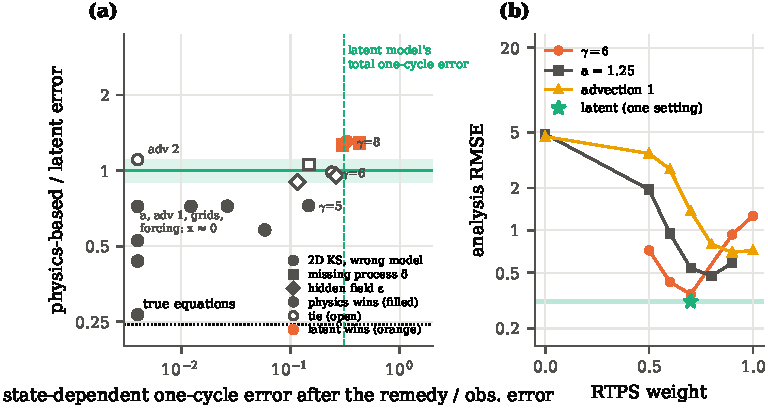
\includegraphics{figures/model_error.pdf}
\caption{Learned versus physics-based filters under model error, 2D KS at $44^2$. (a) The
physics-based filter's error over the latent filter's (three-seed means) against the state-dependent
part of its model's one-cycle forecast error (the part left after bias correction), in units of the
observation error; open: tuned RTPS and localization only; filled: with the best remedy (online
parameter estimation or bias correction); squares: the missing process ($\delta$), diamonds: the hidden
field ($\varepsilon$), each against its own latent model; the band marks $\pm10\%$ of the latent filter, the dotted line
a physics-based filter with the true equations. (b) The physics-based filter's error against its RTPS
weight for three wrong models (log scale; RTPS 0 diverged or was worse than interpolation), and the
latent filter's single setting. In this configuration, below a state-dependent one-cycle error of
about a sixth of the observation error the physics-based filter wins or ties; above it the latent
filter wins, except for the hidden field (diamonds), whose error the physics-based filter largely
removes by estimating the $\nabla^2$ coefficient; and the physics-based filter works only in a narrow
window of its tuning.}
\label{fig:model_error}
\end{figure*}

